% !TeX spellcheck = en_US
\documentclass[authoryear]{elsarticle}
\usepackage{amsmath}
\usepackage{amssymb}
\usepackage{float}
\usepackage{graphicx}
\usepackage{subcaption}
\usepackage{changepage}
\usepackage{url}
\usepackage{xfrac}
\usepackage{booktabs}
\usepackage{rotating}
\usepackage{geometry}
%\usepackage{authblk}
\usepackage{xcolor}
%\usepackage{colortbl}
\usepackage{multirow}
%\usepackage{blindtext}
%\usepackage{mathtools}
%\usepackage{titlesec}
%\setcounter{secnumdepth}{4}
%\usepackage{wasysym}
%\usepackage{cleveref}
%\DeclarePairedDelimiter{\ceil}{\lceil}{\rceil}
\usepackage{lineno}
%\linenumbers
\usepackage{setspace}
\doublespacing
\usepackage[flushleft]{threeparttable}
\usepackage[colorlinks,citecolor=blue,urlcolor=blue]{hyperref} 
%\usepackage{apacite}
\bibliographystyle{elsarticle-harv}

\renewcommand{\thesection}{S\arabic{section}}
\renewcommand{\thefigure}{S\arabic{figure}}
\renewcommand{\thetable}{S\arabic{table}}
\renewcommand{\theequation}{S\arabic{equation}}

\makeatletter
\def\ps@pprintTitle{%
	\let\@oddhead\@empty
	\let\@evenhead\@empty
	\def\@oddfoot{\centerline{\thepage}}%
	\let\@evenfoot\@oddfoot}
\makeatother

% Remove abstract section
\makeatletter
\long\def\pprintMaketitle{\clearpage
	\iflongmktitle\if@twocolumn\let\columnwidth=\textwidth\fi\fi
	\resetTitleCounters
	\def\baselinestretch{1}%
	\printFirstPageNotes
	\begin{center}%
		\thispagestyle{pprintTitle}%
		\def\baselinestretch{1}%
		\Large\@title\par\vskip18pt
		\normalsize\elsauthors\par\vskip10pt
		\footnotesize\itshape\elsaddress\par\vskip36pt
		% \hrule\vskip12pt
		% \ifvoid\absbox\else\unvbox\absbox\par\vskip10pt\fi
		% \ifvoid\keybox\else\unvbox\keybox\par\vskip10pt\fi
		% \hrule\vskip12pt
	\end{center}%
	\gdef\thefootnote{\arabic{footnote}}%
}
\makeatother

\begin{document}
	\begin{frontmatter}
		\title{
			%		Anthropocentric uses of phosphorus: flows quantification and potential for recycling in Ontario
			%	Mapping phosphorus flows in the economic sectors of Ontario and assessing recovery and recycling potential
			Supplementary Information: \\ Mapping of phosphorus flows and analysis of the potential for recovery and reuse in Ontario, Canada
		}
		
		%% Group authors per affiliation:
		\author[ULaval]{Edgar Martín-Hernández}
		%	%\fntext[myfootnote]{Since 1880.}
		\author[Waterloo]{Jorge A. Garcia Hernandez}
		\author[McGill]{Samantha Gangapersad}
		\author[McGill]{Tian Zhao}
		\author[McGill]{Sidney Omelon}
		\author[Waterloo,TheWaterInstitute]{Roy Brouwer}
		\author[ULaval,CentrEau]{Céline Vaneeckhaute\corref{mycorrespondingauthor}}
		\cortext[mycorrespondingauthor]{Corresponding author}
		\ead{celine.vaneeckhaute@gch.ulaval.ca}
		
		\address[ULaval]{BioEngine - Research Team on Green Process Engineering and Biorefineries, Chemical Engineering Department, Université Laval, 1065 Ave. de la Médecine, Québec, QC, G1V 0A6, Canada}
		\address[CentrEau]{CentrEau, Centre de recherche sur l'eau, Université Laval, 1065 Avenue de la Médecine, Québec, QC, G1V 0A6, Canada}
		\address[McGill]{Department of Mining and Materials	Engineering, McGill University, Montréal, Canada}
		\address[Waterloo]{Department of Economics, University of Waterloo, 200 University Avenue West, Waterloo, ON, N2L 3G1, Canada}
		\address[TheWaterInstitute]{The Water Institute, University of Waterloo, 200 University Avenue West, Waterloo, ON, N2L 3G1, Canada}
		
%		\begin{abstract}
%			
%		\end{abstract}
		%	
		%	\begin{keyword}
		%		Quantifying P flows in Ontario's agricultural sector 
		%	\end{keyword}
	\end{frontmatter}
	
	\tableofcontents
	
\newpage
	
\section{Estimation of phosphorus flows}
\subsection{Agriculture and aquaculture sector} \label{section:AgriSector}
Phosphorus flows in the agricultural sector are estimated based on production data of livestock and crop products, as well as on fertilizer application data.
%%For those production data were not available, a number of different methods were used to estimate the P flow based on approaches established in the literature. For example, 
%Phosphorus inflows associated with synthetic fertilizers could be directly estimated based on application data reported in the Fertilizer
%Shipments Survey (FSS) \citep{FertilizerShipments}. Phosphorus in livestock imports and exports is estimated from livestock trading data REF, multiplying the number of animals by the concentration of phosphorus in the different types of livestock REF,

Phosphorus in livestock feeding and manure
%meat and slaughterhouse waste
is estimated based on the number and type of animals reported for Ontario
%at Census Division level
in the Census of Agriculture, including cattle \citep{LivestockCensusCattle}, swine \citep{LivestockCensusPig}, poultry \citep{LivestockCensusPoultry}, and other livestock \citep{LivestockCensusSheep, LivestockCensusOtherLivestock},
%\citep{LivestockCensusCattle,LivestockCensusSheep,LivestockCensusPig,LivestockCensusPoultry,LivestockCensusOtherLivestock},
multiplied by the phosphorus feeding requirements and concentration of phosphorus in manure \citep{NetherlandsCompositions,BrownCompositions, VanStaden2021}.
%and carcasses REF respectively. 
%The Census of Agriculture is published by Statistics Canada every five years (i.e., 2001, 2006, 2011, and 2016) for cattle52 REF, sheep53 REF, swine54 REF, poultry55 REF, and other livestock56 REF, with the exception of rabbits, where data is not available prior to 2009. The number of animals for the years in between census reporting have been estimated using a linear interpolation.
We assumed that the number of animals reported is throughout the year (i.e., the animals culled are replaced by new ones). However, in the case of broilers and turkeys, the number of animals reported by the livestock census have been reduced by a factor of 0.68 (broilers) and 0.80 (turkeys), since these animals have life cycles of 43 and 80 days respectively, meaning barns are empty for 20 days between cycles \citep{yang2007development}.

Phosphorus flows through the imports and exports of animals are estimated using data on animal imports and exports \citep{CattleImportsExports, HogsImportsExports, SheepImportsExports} multiplied by their phosphorus to live weight ratios \citep{NetherlandsCompositions}.

Phosphorus contained in meat and slaughterhouse waste is based on the number of animals slaughtered reported by both federally and provincially licensed meat plants \citep{SlaughterFederalRedMeat, SlaughterFederalPoultry} multiplied by the concentration of phosphorus in carcasses \citep{LivetoCarcassWeight,hayse1973eviscerated,brake1995relationship,NetherlandsCompositions}.

Phosphorus flows associated with the production of milk and eggs are based on provincial production data \citep{EggOntario,MilkOntario}, multiplying these products by their average phosphorus concentration \citep{NutrientValueHealthCanada,chambers2017chicken}.

Phosphorus applied to open fields as synthetic fertilizer is estimated based on the amount of fertilizer products traded to Ontario’s agricultural markets containing phosphorus \citep{FertilizerShipments}. 
%The distribution of phosphorus fertilizers among the Census Division of the province is based on the fraction of fertilized area of each census division, i.e., dividing the reported area of land fertilized for each census division by the total fertilized area of land in Ontario, removing the areas that correspond with greenhouse crops101, 102 103 REF. 
Regarding manure, we assume that all of the manure generated by livestock is applied in crop fields \citep{IROWC_PHandbook}.

The uptake of phosphorus by crops is determined based on the area used in each census division \citep{CensusDivisionOpendatasoft} to grow each type of crops by census division \citep{FieldCropsCensus,FieldVegetablesCensus,GreenhousesCensus} multiplied by the specific yield and phosphorus content for each crop type \citep{USDAHandbook}.  The phosphorus uptake by crops is divided according to whether it is taken up in the grain, fruit or vegetable, or straw and stover components of each type of crop. This is necessary to determine the amount of phosphorus that flows within food or feed (i.e., grains, fruits and vegetables), while straw and stover remain in the field after harvesting as crop residues.

A fraction of the phosphorus applied to crop fields as manure or synthetic fertilizer is lost through erosion, runoff, and drainage. The magnitude of this flow depends on a range of factors, including the amount of phosphorus applied; soil composition, texture, and slope; and precipitations, resulting in a complex and data-intensive process for estimating the phosphorus transported out of the crop fields. As an approximation, we have estimated the phosphorus losses by using export coefficients determined for crop fields in Ontario corrected to account for both surface and subsurface runoffs for synthetic fertilizers (1.267 kg/ha/year), and liquid and solid manure (2.548 kg/ha/year and 1.717 kg/ha/year respectively) \citep{zhang2015tile, wang2018solid,tan2011surface}. In addition, a fraction of the P supplied to crop fields is not taken up by the plants and remains in soil, resulting in the accumulation of P over time as a result of synthetic fertilizer and manure over sustained periods of time, often applying phosphorus in greater quantities than crops require to ensure satisfactory yields \citep{reid2019addressing}. This buildup is often referred to as “legacy P”, and it is estimated as the balance between phosphorus inflows to crop fields (application of manure and synthetic fertilizers) and outflows (crop food and feed products, crop residues, and phosphorus losses by erosion and runoff).

Regarding greenhouse crops, the data available was limited, resulting in an estimation of phosphorus applied as synthetic fertilizers based on the sum of phosphorus uptake by greenhouse crops
%(i.e., tomatoes, peppers, and cucumbers)119
and phosphorus releases from greenhouse irrigation systems also known as greenhouse nutrient feedwater (GNF) systems \citep{GNFOntario}. The phosphorus uptake by greenhouse crops is determined by multiplying the production of greenhouse crops \citep{HorticulturalOntario} by the phosphorus content of each vegetable type \citep{USDAHandbook}. The phosphorus releases from the GNF systems were estimated based on the average concentration of phosphorus in GNF outlet streams for  Ontario, 33.6 mg/L \citep{GreenhouseReleases}, and the total water discharges from GNF systems, assuming that the water discharges are equivalent to 25\% of the total water applied in greenhouses, which corresponds with the worst-case scenario of no water recirculation in the GNF systems \citep{GNFOntario}. The average water consumption in greenhouses in Ontario was assumed to be 1,000 L/m\textsuperscript{2}/year \citep{GrowingVeggiesOntario}. We have also estimated the phosphorus releases from the seasonal workers living in households in the vicinity of the greenhouses that may use septic systems, considering that the seasonal labour force in Ontario greenhouses is estimated to be 6,699 workers \citep{GreenhouseWorkers}, and an average phosphorus load rate of 0.0156 kg P/person/week from septic systems \citep{oldfield2020estimation}.

%Phosphorus in aquaculture are mainly due to supply of feed as part of fish feed the grow of trouts, part of which is uptake by fishes, while the rest of phosphorus is released into aquatic ecosystems since aquaculture effluents are directly discharged to the environment
Phosphorus enters aquaculture systems as fish feed, primarily in the growth of trouts. A fraction of this phosphorus goes to the fish and the remainder is discharged into aquatic ecosystems as aquaculture effluents
\citep{OntarioAquaculture}. 
The total phosphorus in fish produced in Ontario
%supplied to aquaculture as fish feed is taken from, while the phosphorus uptakes by fishes are 
is calculated by multiplying the fish production \citep{StatisticsCanadaAquaculture} by their phosphorus content \citep{CanadianNutrientFile}, while the phosphorus content in the aquaculture waste effluents of Ontario is estimated to be 10 kg of phosphorus per ton of fish produced \citep{bureau2003chemical}. The phosphorus in Ontario fish feed that is supplied to aquaculture, is estimated to be the sum of the phosphorus in the fish produced and the phosphorus in aquaculture effluent.

\subsection{Industrial sector}
Phosphorus flows through imports, production, exports and waste for the food, steel, and forestry industries of Ontario were mapped.

%{\color{red} REVISAR POR SIDNEY }
Processed food imports and exports
are estimated scaling each type of food 
%available in Canada \citep{FoodAvailableCanada} 
traded in Canada \citep{TradeDataOnlineCanada}
with the population of Ontario \citep{PopulationCanada}.
%and then subtracting the amount of each type of food produced within Ontario.
The phosphorus contained in each type of imported and exported food is estimated by multiplying the amount of each type of traded food by its phosphorus content \citep{CanadianNutrientFile}. Phosphorus flows in the form of food and organic waste are based on applying food loss factors for the steps associated with food processing, from the production of food raw materials to consumption \citep{FoodLossesFAO}, considering the food production and import values estimated in Section \ref{section:AgriSector}.

The steel industry is the first non-food sector in terms of phosphorus use. The main phosphorus inflows of steel manufacturing are associated with the use of iron ore, coal, and coke, while the
%main outflow of phosphorus is within slag, which remove most of the impurities from steel, including phosphorus.
main outflow of phosphorus is within slag, a by-product of steelmaking. During steelmaking, most of the impurities, including phosphorus, separate into the slag phase.
It must be noted that, although some minor amounts of phosphorus can be desired in steel for making anti-corrosion surface coatings, it is largely considered an impurity in the steel manufacturing process. Phosphorus in these flows is estimated by multiplying their average phosphorus content (0.06\% P in iron ore, 0.05\% P for coal, 0.4\% P in slag, and 0.01\% in steel) \citep{yokoyama2007separation} by the steel production capacity of the facilities located in Ontario \citep{CheminfoServices, AlgomaSteel, Stelco, PFlows_Ontario} and the imports and exports of these materials \citep{WorldIntegratedTradeSolution, InterprovincialImportsExports}. The P in slag is estimated using component balancing.

Phosphorus flows in Ontario's forestry industry include wood harvesting, wood products manufacturing, as well as the production of pulp and paper. The estimation of these phosphorus flows are the result of multiplying the production data of wood, wood products, pulp and paper, and their respective imports, exports, and waste streams \citep{CanadianForestServiceStatistics, InterprovincialImportsExports}, by their average phosphorus content.
%which is assumed to be 0.01\% for wood \citep{sardans2013tree} and 0.005\% for pulp and paper products.
The average phosphorus content used for wood is 0.01\% \citep{sardans2013tree} and 0.005\% is estimated for pulp and paper products, using component balancing.

%The general chemical facilities located in Ontario report 350 t/year of phosphorus as waste \citep{PFlows_Ontario}, in addition of imports and exports of chemical products. 
The local production of phosphorus is assumed to be negligible since phosphorus is not mined or refined in Ontario. Synthetic phosphorus fertilizer and phosphorus chemical imports are estimated similar to food imports.  The phosphorus fertilizer imports are accounted for in the agricultural section. Chemical facilities located in Ontario report 350 t/year of phosphorus as waste \citep{PFlows_Ontario}.
However,
%there exist a significant fraction of phosphorus used in the industrial sector that cannot be tracked due to the lack of data.
a significant fraction of phosphorus used in the industrial sector cannot be tracked due to the lack of data.
%Regarding other industrial activities which could involve the use of phosphorus, the local production of phosphorus is assumed to be negligible since phosphorus is not mined or refined in Ontario, and the synthetic phosphorus fertilizer imports are accounted in the agricultural section.

%{\color{red}Ask sidney what to do with food industry, and pet feed. My approach is to merge all of them as it is currently in the figure, but confirm with her}

%\newpage
\subsection{Slaughter industry}
Table \ref{table:SlaughterAnimals} collects the number of animals slaughtered and the phosphorus in slaughterhouse waste in the province of Ontario for year 2019.

\begin{table}[h]
	\centering
	\caption{Truncated normal distribution fitting parameters for the distribution of cAFOs sizes in regions of the Great Lakes area.} \label{table:SlaughterAnimals}
	\resizebox{0.99\columnwidth}{!}{
		%		\begin{threeparttable}
			\begin{tabular}{@{}lcccccc@{}}
				\toprule
				& Cattle  & Swine     & Sheep   & Rabbit        & Poultry                                                                         & Total                        \\ \midrule
				\begin{tabular}[c]{@{}l@{}}Animals slaughtered in federally\\ licensed facilities (heads, 2019)\end{tabular}    & 628,366 & 4,010,926 & 84,721  & Not available & \multirow{2}{*}{\begin{tabular}[c]{@{}c@{}}238,979,246 \\ (total)\end{tabular}} & \multirow{2}{*}{244,663,410} \\
				\begin{tabular}[c]{@{}l@{}}Animals slaughtered in provincially\\ licensed facilities (heads, 2019)\end{tabular} & 99,561  & 368,267   & 266,946 & 225,377       &                                                                                 &                              \\
				\begin{tabular}[c]{@{}l@{}}P flows through slaughterhouse\\ waste in t (2019)\end{tabular}                      & 2,222   & 621       & 42      & 7.3           & 904                                                                             & 3,796.6                      \\ \bottomrule
			\end{tabular}
			%			\begin{tablenotes}
				%				\footnotesize
				%				\item 1: \citet{MilkOntario}
				%			\end{tablenotes}
			%	\end{threeparttable}
	}
\end{table}


	
\section{Phosphorus recovery processes}	
\subsection{Scaling CAFOs phosphorus recovery processes}
We refer the reader to \citet{martin2021geospatial} for a detailed description on estimating the phosphorus recovery costs of processes from phosphorus recovery from livestock facilities. Capital costs are annualized through the application of an annual capital charge ratio $\left( ACCR\right)$ as defined by \citet{towler2013chemical}, shown in Eq. \ref{eq:ACCR}, assuming a typical interest rate $i$ of 5\% and a plant lifetime $n$ of 20 years.
\begin{align}
	& ACCR = \frac{i\left( 1 + i\right)^n }{\left(1+i \right)^n -1 } \label{eq:ACCR}
\end{align}

\subsection{Scaling municipal wastewater phosphorus recovery processes}
Data on processes for phosphorus recovery from municipal wastewater is taken from \citet{egle_phosphorus_2016}. We assume that, similarly to other industrial activities \citep{dysert2005so}, the phosphorus recovery cost from municipal wastewater in function of the plant capacity shows an exponential behavior. In consequence, the cost-to-capacity method \citep{baumann2014cost} is used to estimate phosphorus recovery cost from municipal wastewater in function of the plant capacity, as shown in Eq. \ref{eq:CostoToCapacity1}, where $x$ denotes the scale factor 'facility 2' refers to the facility which cost is required while 'facility 1' denotes the facility whose data is known. The scale factor $x$ is estimated based on the data for different capacities reported by \citet{egle_phosphorus_2016} through the transformation of Eq. \ref{eq:CostoToCapacity1} by applying natural logarithms to both sides of the equation, as shown in Eq. \ref{eq:CostoToCapacityLinearization}. The scale factor obtained are shown in Table \ref{table:WWTPsPRecTechsScaleFactor}. The capacity magnitude has been normalized to the mass of phosphorus recovered.

\begin{table}[h]
	\centering
	\caption{Estimation of scale factors for municipal wastewater phosphorus recovery systems.} \label{table:WWTPsPRecTechsScaleFactor}
	\resizebox{0.99\columnwidth}{!}{
		%		\begin{threeparttable}
		\begin{tabular}{@{}ccccccc@{}}
			\toprule
			Inflow                                                                           & Technology        & Type                       & \begin{tabular}[c]{@{}c@{}}P recovery potential\\ (\% related to inflow)\end{tabular} & \begin{tabular}[c]{@{}c@{}}P inflow\\ (kg P/year)\end{tabular} & \begin{tabular}[c]{@{}c@{}}Annual processing\\ cost (EUR)\end{tabular} & \begin{tabular}[c]{@{}c@{}}Scale factor \\  $x$  \end{tabular}                    \\ \midrule
			\multirow{12}{*}{\begin{tabular}[c]{@{}c@{}}WWTPs\\ (liquid phase)\end{tabular}} & \multirow{2}{*}{Crystalactor}      & \multirow{2}{*}{Struvite/Calcium phosphate} & \multirow{2}{*}{38 }                                                                                   & 65700                                                          & 305920                                                      & \multirow{2}{*}{0.59} \\
			&      &  &                                                                                    & 328500                                                         & 795893                                                      &                                    \\
			& \multirow{2}{*}{Ostara Pearl}      & \multirow{2}{*}{Struvite}                   & \multirow{2}{*}{20}                                                                                 & 65700                                                          & 130856                                                      & \multirow{2}{*}{0.36} \\
			&       &                    &                                                                                     & 328500                                                         & 235234                                                      &                                    \\
			& \multirow{2}{*}{P-RoC}             & \multirow{2}{*}{Calcium phosphate}          & \multirow{2}{*}{27}                                                                                    & 65700                                                          & 75970                                                       & \multirow{2}{*}{0.78}  \\
			&          &           &                                                                                     & 328500                                                         & 266025                                                      &                                    \\
			& \multirow{2}{*}{REM-NUT}           & \multirow{2}{*}{Struvite}                   & \multirow{2}{*}{47}                                                                                    & 65700                                                          & 977933                                                      & \multirow{2}{*}{0.94} \\
			&            &                    &                                                                                     & 328500                                                         & 4417171                                                     &                                    \\
			& \multirow{2}{*}{AirPrex}           & \multirow{2}{*}{Struvite}                  & \multirow{2}{*}{15}                                                                                    & 65700                                                          & 74195                                                       & \multirow{2}{*}{0.38}  \\
			&            &                    &                                                                                     & 328500                                                         & 137693                                                      &                                    \\
			& \multirow{2}{*}{PRISA}             & \multirow{2}{*}{Struvite}                   & \multirow{2}{*}{18}                                                                                   & 65700                                                          & 186923                                                      & \multirow{2}{*}{0.43} \\
			&              &                    &                                                                                     & 328500                                                         & 371578                                                      &                                    \\ \cmidrule(lr){2-7}
			\multirow{10}{*}{WWTPs}                                                          & \multirow{2}{*}{Stuttgart process} & \multirow{2}{*}{Struvite}                   & \multirow{2}{*}{40}                                                                                    & 65700                                                          & 581730                                                      & \multirow{2}{*}{0.89}   \\ 
			&  &                    &                                                                                     & 328500                                                         & 2419407                                                     &                                    \\
			& \multirow{2}{*}{Gifhorn process}   & \multirow{2}{*}{Struvite}                   & \multirow{2}{*}{40}                                                                                    & 65700                                                          & 400384                                                      & \multirow{2}{*}{0.82} \\
			&     &                    &                                                                                     & 328500                                                         & 1491509                                                     &                                    \\
			& \multirow{2}{*}{PHOXNAN}           & \multirow{2}{*}{Struvite}                   & \multirow{2}{*}{51}                                                                                    & 65700                                                          & 891667                                                      & \multirow{2}{*}{0.84} \\
			&            &                    &                                                                                     & 328500                                                         & 3468902                                                     &                                    \\
			& \multirow{2}{*}{Aqua Reci}         & \multirow{2}{*}{Calcium phosphate}          & \multirow{2}{*}{61}                                                                                    & 65700                                                          & 939605                                                      & \multirow{2}{*}{0.82}  \\
			&         &            &                                                                                     & 328500                                                         & 3529595                                                     &                                    \\
			& \multirow{2}{*}{MEPHREC}           & \multirow{2}{*}{P rich slag}                & \multirow{2}{*}{68}                                                                                    & 65700                                                          & 1154473                                                     & \multirow{2}{*}{0.61} \\
			&            &                &                                                                                     & 657000                                                         & 4715866                                                     &                                    \\ \bottomrule
		\end{tabular}
		%			\begin{tablenotes}
		%				\footnotesize
		%				\item 1: \citet{MilkOntario}
		%			\end{tablenotes}
		%	\end{threeparttable}
	}
\end{table}
\begin{align}
	& \frac{\text{Cost}_{\text{facilitiy 2}}}{\text{Cost}_{\text{facilitiy 1}}} = \left( \frac{\text{Capacity}_{\text{facilitiy 2}}}{\text{Capacity}_{\text{facilitiy 1}}} \right)^x \label{eq:CostoToCapacity1}\\
	& x = \frac{\text{ln} \left(\frac{\text{Cost}_{\text{facilitiy 2}}}{\text{Cost}_{\text{facilitiy 1}}} \right) }{\text{ln} \left( \frac{\text{Capacity}_{\text{facilitiy 2}}}{\text{Capacity}_{\text{facilitiy 1}}}\right) } \label{eq:CostoToCapacityLinearization}
\end{align}

%\appendix

%\vspace{5cm}
\subsection{Phosphorus recovery technologies techno-economic data}

Table \ref{table:TechParam} collects the main specifications of the phosphorus recovery technologies considered in this work, including the estimation of phosphorus recovery cost.

\begin{sidewaystable}[!htbp]%[!htbp]
%	\subsection{Phosphorus recovery technologies techno-economic data}
	%\begin{table}[!htbp]%[!htbp]
	\centering
	\caption{Phosphorus recovery technologies considered in the study. For the treatment of manure we assumed that the units for the separation of the solid and liquid phases is already implemented in the livestock operations. $F$ denotes the phosphorus recovered as $\sfrac{\text{kg P}_{\text{recovered}}}{\text{year}}$, while $\lceil x \rceil$ represent the ceiling function applied to $x$. The definition of annual capital charge ratio $\left( ACCR\right)$ can be found in the Supplementary Material, Section 1.1. Refs: 1: \protect\citet{martin2021geospatial},
		2: \protect\citet{jupp2021phosphorus},
		3: \protect\citet{egle_phosphorus_2016},
		4: \protect\citet{schoumans2010phosphorus},
		5: \protect\citet{szogi2008phosphorus},
		6: \protect\citet{Pearl2Kcost2},
		7: \protect\citet{zagklis2020assessing},
		8: \protect\citet{fernandez2022phosphorus},
		9: \protect\citet{ohtake2019phosphorus},
		10: \protect\citet{sharma2021life}} \label{table:TechParam}
	\resizebox{1.09\columnwidth}{!}{
		\begin{threeparttable}
			\begin{tabular}{@{}cccccccccc@{}}
				\toprule
				Sector                        & Inflow                                                                                                                                                  & Pretreatment                                                                     & \begin{tabular}[c]{@{}c@{}}Pretreatment cost\\ (EUR/kg P\textsubscript{recovered})\end{tabular} & Technology                                                                               & Type                                                                              & \begin{tabular}[c]{@{}c@{}}P recovery potential\\ (\% related to inflow)\end{tabular} & P recovery cost (EUR/kg P recovered) & TRL                                   & Ref tech \\ \midrule
				\multirow{27}{*}{Agriculture} & \multirow{10}{*}{\begin{tabular}[c]{@{}c@{}}Cattle and swine manure, \\ liquid phase\\ (30\% of total manure P)\end{tabular}}                               &
				%				\begin{tabular}[c]{@{}c@{}}Solid-liquid separation\\ (screw press)\end{tabular}
				Solid-liquid separation
				&         -
				%				See [1]
				& Multiform                                                                                & Struvite                                                                          & 60                                                                                    & $25.7 + 1.10 \cdot 10^6 \cdot \lceil 1.19 \cdot 10^{-4} \cdot F \rceil \cdot ACCR \cdot \frac{1}{F}$                                 & 9                                                            & [1]    \\
				&                                                                                                                                                         & Solid-liquid separation
				%				\begin{tabular}[c]{@{}c@{}}Solid-liquid separation\\ (screw press)\end{tabular} 
				& -
				%				See [1]
				& Crystalactor                                                                             & \begin{tabular}[c]{@{}c@{}}Struvite/\\ calcium phosphate\end{tabular}                                           & 60                                                                                    & $3.53 + \left( 2.30 \cdot 10^6 + 0.71 \cdot \lceil 3.32 \cdot 10^{-5} \cdot F \rceil\right)\lceil 3.32 \cdot 10^{-5} \cdot F \rceil \cdot ACCR \cdot \frac{1}{F} $                                  & 9                                                            &[1]          \\
				&                                                                                                                                                         & 
				Solid-liquid separation
				%				\begin{tabular}[c]{@{}c@{}}Solid-liquid separation\\ (screw press)\end{tabular}
				&   -
				%				See [1]
				& Ostara Pearl 500                                                                             & Struvite                                                                          & 60                                                                                    &  $12.57 + 2.30 \cdot 10^6 \cdot \lceil 7.02 \cdot 10^{-5} \cdot F \rceil \cdot ACCR \cdot \frac{1}{F}$                                & 9                                                            & [1]         \\
				& & Solid-liquid separation
				%				\begin{tabular}[c]{@{}c@{}}Solid-liquid separation\\ (screw press)\end{tabular}
				&     -
				%				See [1]
				& Ostara Pearl 2K                                                                             & Struvite                                                                          & 60                                                                                    & $12.57 + 3.10 \cdot 10^6 \cdot \lceil 1.83 \cdot 10^{-5} \cdot F \rceil \cdot ACCR \cdot \frac{1}{F}$                                 & 9                                                            &  [1]        \\
				& & Solid-liquid separation
				%				\begin{tabular}[c]{@{}c@{}}Solid-liquid separation\\ (screw press)\end{tabular} 
				&      -
				%				See [1]
				& Ostara Pearl 10K                                                                             & Struvite                                                                          & 60                                                                                    &  $12.57 + 10.00 \cdot 10^6 \cdot \lceil 3.65 \cdot 10^{-6} \cdot F \rceil \cdot ACCR \cdot \frac{1}{F}$                                  & 9                                                            &   [1]       \\
				&                                                                                                                                                         & Solid-liquid separation
				%				\begin{tabular}[c]{@{}c@{}}Solid-liquid separation\\ (screw press)\end{tabular} 
				&              -
				%				See [1]
				& Nuresys                                                                                  & Struvite                                                                          & 60                                                                                    & $10.37 + 1.38 \cdot 10^6 \cdot \lceil 2.24 \cdot 10^{-5} \cdot F \rceil \cdot ACCR \cdot \frac{1}{F}$                                  & 9                                                            & [1]         \\
				%			&                                                                                                                                                         & \begin{tabular}[c]{@{}c@{}}Solid-liquid separation\\ ( screw press)\end{tabular} &                                        & P-RoC                                                                                    & Calcium phosphate                                                                 & 60                                                                                    & 36.8                                 & 6                                                            &          \\
				&                                                                                                                                                         & Solid-liquid separation
				%				\begin{tabular}[c]{@{}c@{}}Solid-liquid separation\\ (screw press)\end{tabular}
				&    -
				%				See [1]
				& MAPHEX                                                                                   & Solid                                                                             & 90                                                                                    & $184.67 + 0.30 \cdot 10^6 \cdot \lceil 2.47 \cdot 10^{-4} \cdot F \rceil \cdot ACCR \cdot \frac{1}{F}$                                  & 6                                                            &     [1]     \\ \cmidrule(l){2-10}
				& \multirow{7}{*}{\begin{tabular}[c]{@{}c@{}}Cattle and swine manure, \\ solid phase\\ (70\% of total manure P)\end{tabular}}                                & Incineration                                                                     & 8.9                                    & EcoPhos                                                                                  & Phosphoric acid                                                                   & 82                                                                                    & 4.5                                  & 6                                                            & [2,3,4]    \\ 
				&                                                                                                                                                         & Incineration                                                                     & 8.9                                    & AshDec depollution                                                                       & Calcium phosphate                                                                 & 86                                                                                    & 1.8                                  & 6                                                            &   [2,3,4] \\
				&                                                                                                                                                         & Incineration                                                                     & 8.9                                    & AshDec Rhenania                                                                          & Calcium phosphate                                                                 & 86                                                                                    & 1.9                                  & 6                                                            &   [2,3,4] \\
				&                                                                                                                                                         & Incineration                                                                     & 8.9                                    & PASCH                                                                                    & Calcium phosphate                                                                 & 79                                                                                    & 4.7                                  & 6                                                            &  [2,3,4]  \\
				&                                                                                                                                                         & Incineration                                                                     & 8.9                                    & LEACHPHOS                                                                                & Calcium phosphate                                                                 & 78                                                                                    & 5.1                                  & 9                                                            &  [2,3,4]  \\
				&                                                                                                                                                         & Incineration                                                                     & 8.9                                    & RecoPhos                                                                                 & Mineral                                                                           & 87                                                                                    & 2.5                                  & 9                                                            & [2,3,4]   \\
				&                                                                                                                                                         & Incineration                                                                     & 8.9                                    & Thermophos                                                                               & P4                                                                                & 81                                                                                    & 2.7                                  & 9                                                            &  [2,3,4]  \\ \cmidrule(l){2-10}
				& Poultry litter                                                                                                                                          & -                                                                               & -                                     & Quick wash                                                                               & Solid precipitate                                                                 & 70                                                                                    & 4.4                                  & 4-6   &    [5]      \\ \cmidrule(l){2-10}
				& \multirow{4}{*}{\begin{tabular}[c]{@{}c@{}}Slaughterhouse waste, \\ liquid phase\\ (14\% of total slaughterhouse P)\end{tabular}}                    & -                                                                               & -                                     & Multiform                                                                                & Struvite                                                                          & 84                                                                                    & $22.6 + 1.10 \cdot 10^6 \cdot \lceil 1.05 \cdot 10^{-4} \cdot F \rceil \cdot ACCR \cdot \frac{1}{F}$                                 & 9                                                           &  [6]  \\
				&                                                                                                                                                         & -                                                                               & -                                     & Ostara Pearl 500                                                                             & Struvite                                                                          & 58                                                                                    & $15.60 + 2.30 \cdot 10^6 \cdot \lceil 8.70 \cdot 10^{-5} \cdot F \rceil \cdot ACCR \cdot \frac{1}{F}$                                 & 9                                                            &     [6]     \\
				&                                                                                                                                                         & -                                                                               & -                                     & Ostara Pearl 2K                                                                             & Struvite                                                                          & 58                                                                                    & $15.60 + 3.10 \cdot 10^6 \cdot \lceil 2.26 \cdot 10^{-5} \cdot F \rceil \cdot ACCR \cdot \frac{1}{F}$                                 & 9                                                            &    [6]      \\
				&                                                                                                                                                         & -                                                                               & -                                     & Ostara Pearl 10K                                                                             & Struvite                                                                          & 58                                                                                    & $15.60 + 10.00 \cdot 10^6 \cdot \lceil 4.53 \cdot 10^{-6} \cdot F \rceil \cdot ACCR \cdot \frac{1}{F}$                                 & 9                                                            &    [6]      \\ \cmidrule(l){2-10}
				& \multirow{7}{*}{\begin{tabular}[c]{@{}c@{}}Slaughterhouse waste, \\ solid phase\\ (86\% of total slaughterhouse P)\end{tabular}}                     & Incineration                                                                     & 14.6                                   & EcoPhos                                                                                  & Phosphoric acid                                                                   & 82                                                                                    & 4.5                                  & 6                                                            &   [2,3,7] \\
				&                                                                                                                                                         & Incineration                                                                     & 14.6                                   & AshDec depollution                                                                       & Calcium phosphate                                                                 & 86                                                                                    & 1.8                                  & 6                                                            &  [2,3,7]  \\
				&                                                                                                                                                         & Incineration                                                                     & 14.6                                   & AshDec Rhenania                                                                          & Calcium phosphate                                                                 & 86                                                                                    & 1.9                                  & 6                                                            &   [2,3,7] \\
				&                                                                                                                                                         & Incineration                                                                     & 14.6                                   & PASCH                                                                                    & Calcium phosphate                                                                 & 79                                                                                    & 4.7                                  & 6                                                            &   [2,3,7] \\
				&                                                                                                                                                         & Incineration                                                                     & 14.6                                   & LEACHPHOS                                                                                & Calcium phosphate                                                                 & 78                                                                                    & 5.1                                  & 9                                                            &  [2,3,7]  \\
				&                                                                                                                                                         & Incineration                                                                     & 14.6                                   & RecoPhos                                                                                 & Mineral                                                                           & 87                                                                                    & 2.5                                  & 9                                                            &  [2,3,7]  \\
				&                                                                                                                                                         & Incineration                                                                     & 14.6                                   & Thermophos                                                                               & P4                                                                                & 81                                                                                    & 2.7                                  & 9                                                            &  [2,3,7]  \\ \cmidrule(l){1-10}
				\multirow{36}{*}{\begin{tabular}[c]{@{}c@{}}Urban \& \\ industrial\end{tabular}}       & \multirow{10}{*}{\begin{tabular}[c]{@{}c@{}}WWTPs\\ (liquid phase,\\ 14\% of total wastewater P)\end{tabular}}                                                                         & -                                                                               & -                                     & Crystalactor                                                                             & \begin{tabular}[c]{@{}c@{}}Struvite/\\ Calcium phosphate\end{tabular}                                                         & 38                                                                                    & $305,920 \cdot \left( \frac{F}{24,966} \right)^{0.59} \cdot \frac{1}{F}$                                 & 9                                                            &     [3]     \\
				&                                                                                                                                                         & -                                                                               & -                                     & Ostara Pearl                                                                             & Struvite                                                                          & 20                                                                                    & $130,856 \cdot \left( \frac{F}{13,140} \right)^{0.36} \cdot \frac{1}{F}$                                  & 9                                                            &   [3]       \\
				&                                                                                                                                                         & -                                                                               & -                                     & P-RoC                                                                                    & Calcium phosphate                                                                 & 27                                                                                    & $75,970 \cdot \left( \frac{F}{17,739} \right)^{0.78} \cdot \frac{1}{F}$                                  & 6                                                            &    [3]      \\
				&                                                                                                                                                         & -                                                                               & -                                     & REM-NUT                                                                                  & Struvite                                                                          & 47                                                                                    & $977,933 \cdot \left( \frac{F}{30,879} \right)^{0.94} \cdot \frac{1}{F}$                                 & 6                                                            &   [3]       \\
				&                                                                                                                                                         & -                                                                               & -                                     & AirPrex                                                                                  & Struvite                                                                          & 15                                                                                    & $74,195 \cdot \left( \frac{F}{9,855} \right)^{0.38} \cdot \frac{1}{F}$                                  & 9                                                            &     [3]     \\
				&                                                                                                                                                         & -                                                                               & -                                     & PRISA                                                                                    & Struvite                                                                          & 18                                                                                    & $186,923 \cdot \left( \frac{F}{11,826} \right)^{0.43} \cdot \frac{1}{F}$                                  & 6                                                            &     [3]     \\ \cmidrule(l){2-10}
				& \multirow{8}{*}{\begin{tabular}[c]{@{}c@{}}WWTPs \\ (sewage sludge,\\ 86\% of total wastewater P)\end{tabular}}                                                       & -                                                                               & -                                     & Stuttgart process                                                                        & Struvite                                                                          & 40                                                                                    & $581,730 \cdot \left( \frac{F}{26,280} \right)^{0.89} \cdot \frac{1}{F}$                                 & 9                                                            &   [3]       \\
				&                                                                                                                                                         & -                                                                               & -                                     & Gifhorn process                                                                          & Struvite                                                                          & 40                                                                                    & $400,384 \cdot \left( \frac{F}{26,280} \right)^{0.82} \cdot \frac{1}{F}$                                    & 9                                                            &   [3]       \\
				&                                                                                                                                                         & -                                                                               & -                                     & PHOXNAN                                                                                  & Struvite                                                                          & 51                                                                                    & $891,667 \cdot \left( \frac{F}{33,507} \right)^{0.84} \cdot \frac{1}{F}$                                 & 6                                                            &    [3]      \\
				&                                                                                                                                                         & -                                                                               & -                                     & Aqua Reci                                                                                & Calcium phosphate                                                                 & 61                                                                                    & $939,605 \cdot \left( \frac{F}{40,077} \right)^{0.82} \cdot \frac{1}{F}$                                 & 6                                                            &    [3]      \\
				&                                                                                                                                                         & -                                                                               & -                                     & MEPHREC                                                                                  & P rich slag                                                                       & 68                                                                                    & $1,154,473 \cdot \left( \frac{F}{44,676} \right)^{0.61} \cdot \frac{1}{F}$                                 & 6                                                            &    [3]      \\ \cmidrule(l){2-10}
				& \multirow{7}{*}{\begin{tabular}[c]{@{}c@{}}WWTPs \\ (sewage sludge ash SSA,\\ 86\% of total wastewater P)\end{tabular}}                                               & Incineration                                                                     & 8                                      & EcoPhos                                                                                  & Phosphoric acid                                                                   & 82                                                                                    & 4.5                                  & 6                                                            &    [3]      \\
				&                                                                                                                                                         & Incineration                                                                     & 8                                      & AshDec depollution                                                                       & Calcium phosphate                                                                 & 86                                                                                    & 1.8                                  & 6                                                            &    [3]      \\
				&                                                                                                                                                         & Incineration                                                                     & 8                                      & AshDec Rhenania                                                                          & Calcium phosphate                                                                 & 86                                                                                    & 1.9                                  & 6                                                            &     [3]     \\
				&                                                                                                                                                         & Incineration                                                                     & 8                                      & PASCH                                                                                    & Calcium phosphate                                                                 & 79                                                                                    & 4.7                                  & 6                                                            &     [3]     \\
				&                                                                                                                                                         & Incineration                                                                     & 8                                      & LEACHPHOS                                                                                & Calcium phosphate                                                                 & 78                                                                                    & 5.1                                  & 9                                                            &     [3]     \\
				&                                                                                                                                                         & Incineration                                                                     & 8                                      & RecoPhos                                                                                 & Mineral                                                                           & 87                                                                                    & 2.5                                  & 9                                                            &      [3]    \\
				&                                                                                                                                                         & Incineration                                                                     & 8                                      & Thermophos                                                                               & P4                                                                                & 81                                                                                    & 2.7                                  & 9                                                            &    [3]      \\ \cmidrule(l){2-10}
				& \multirow{5}{*}{\begin{tabular}[c]{@{}c@{}}Organic municipal\\ \& food waste\end{tabular}}
				%			& -                                                                               & -                                     & \begin{tabular}[c]{@{}c@{}}Chemical extraction and\\ Struvite precipitation\end{tabular} & Struvite                                                                          & 94                                                                                    & 24.8                                 & 3  &  [8]        \\                                              & & Incineration                                                                     & 6.43                                      & EcoPhos                                                                                  & Phosphoric acid                                                                   & 82                                                                                    & 4.5                                  & 6                                                            &   [3,9,10]       \\
				%			&                                                                                                                                                         & Incineration                                                                     & 6.43                                      & AshDec depollution                                                                       & Calcium phosphate                                                                 & 86                                                                                    & 1.8                                  & 6                                                            &    [3,9,10]      \\
				%			&
				& Incineration                                                                     & 6.43                                      & AshDec Rhenania                                                                          & Calcium phosphate                                                                 & 86                                                                                    & 1.9                                  & 6                                                            &    [3,9,10]      \\
				&                                                                                                                                                         & Incineration                                                                     & 6.43                                      & PASCH                                                                                    & Calcium phosphate                                                                 & 79                                                                                    & 4.7                                  & 6                                                            &     [3,9,10]     \\
				&                                                                                                                                separation                         & Incineration                                                                     & 6.43                                      & LEACHPHOS                                                                                & Calcium phosphate                                                                 & 78                                                                                    & 5.1                                  & 9                                                            &      [3,9,10]    \\
				&                                                                                                                                                         & Incineration                                                                     & 6.43                                      & RecoPhos                                                                                 & Mineral                                                                           & 87                                                                                    & 2.5                                  & 9                                                            &     [3,9,10]     \\
				&                                                                                                                                                         & Incineration                                                                     & 6.43                                      & Thermophos                                                                               & P4                                                                                & 81                                                                                    & 2.7                                  & 9                                                            &     [3,9,10]     \\ 
				%			\cmidrule(l){1-10}
				%			\multirow{2}{*}{Industrial}   & \multirow{2}{*}{Steel production}                                                                                                                       & -                                                                               & -                                     & Reductive melting                                                                        & \begin{tabular}[c]{@{}c@{}}I have doubts if this P\\ can be recycled\end{tabular} & ?                                                                                     &                                      & 5                                                             &          \\
				%			&                                                                                                                                                         & -                                                                               & -                                     & \begin{tabular}[c]{@{}c@{}}Selective leaching–chemical\\ Precipitation\end{tabular}      & \begin{tabular}[c]{@{}c@{}}I have doubts if this P\\ can be recycled\end{tabular} & ?                                                                                     &                                      & 4                                                             &          
				%			\\
				\bottomrule
				%			\cmidrule(l){3-10} 
			\end{tabular}
			%					\begin{tablenotes}
				%						\footnotesize
				%						\item 1: \citet{martin2021geospatial}
				%						\item 2: \citet{jupp2021phosphorus}
				%						\item 3: \citet{egle_phosphorus_2016}
				%						\item 4: \citet{schoumans2010phosphorus}
				%						\item 5: \citet{szogi2008phosphorus}
				%						\item 6: \citet{Pearl2Kcost2}
				%						\item 7: \citet{zagklis2020assessing}
				%						\item 8: \citet{fernandez2022phosphorus}
				%						\item 9: \citet{ohtake2019phosphorus}
				%						\item 10: \citet{sharma2021life}
				%					\end{tablenotes}
		\end{threeparttable}
	}
\end{sidewaystable}



%\subsection{Specifications of phosphorus recovery technologies}
%Table \ref{table:TechParam} collects the main specifications of the phosphorus recovery technologies considered in this work, including the estimation of phosphorus recovery cost.
%
%%\begin{table}[h]
%\begin{sidewaystable}[!htbp]
%	\centering
%	\caption{Phosphorus recovery techniques considered in the study. $F$ denotes the phosphorus recovered as $\sfrac{\text{kg P}_{\text{recovered}}}{\text{year}}$, while $\lceil x \rceil$ represent the ceiling function applied to $x$. The definition of annual capital charge ratio $\left( ACCR\right)$ can be found in the Supplementary Material, Section 1.1. Refs: [1]: \protect\citet{martin2021geospatial},
%		[2]: \protect\citet{jupp2021phosphorus},
%		[3]: \protect\citet{egle_phosphorus_2016},
%		[4]: \protect\citet{schoumans2010phosphorus},
%		[5]: \protect\citet{szogi2008phosphorus},
%		[6]: \protect\citet{Pearl2Kcost2},
%		[7]: \protect\citet{zagklis2020assessing},
%		[8]: \protect\citet{fernandez2022phosphorus},
%		[9]: \protect\citet{ohtake2019phosphorus},
%		[10]: \protect\citet{sharma2021life}} \label{table:TechParam}
%	\resizebox{1.08\columnwidth}{!}{
%		\begin{threeparttable}
%			\begin{tabular}{@{}cccccccccc@{}}
%				\toprule
%				Sector                        & Inflow                                                                                                                                                  & Pretreatment                                                                     & \begin{tabular}[c]{@{}c@{}}Pretreatment cost\\ (EUR/kg P\textsubscript{recovered})\end{tabular} & Technology                                                                               & Type                                                                              & \begin{tabular}[c]{@{}c@{}}P recovery potential\\ (\% related to inflow)\end{tabular} & P recovery cost (EUR/kg P recovered) & TRL                                   & Ref tech \\ \midrule
%				\multirow{27}{*}{Agriculture} & \multirow{10}{*}{\begin{tabular}[c]{@{}c@{}}Cattle and swine manure, \\ liquid phase\\ (30\% of total manure P)\end{tabular}}                               & \begin{tabular}[c]{@{}c@{}}Solid-liquid separation\\ (screw press)\end{tabular} &        See [1]                                & Multiform                                                                                & Struvite                                                                          & 60                                                                                    & $25.7 + 1.10 \cdot 10^6 \cdot \lceil 1.19 \cdot 10^{-4} \cdot F \rceil \cdot ACCR \cdot \frac{1}{F}$                                 & 9                                                            & [1]    \\
%				&                                                                                                                                                         & \begin{tabular}[c]{@{}c@{}}Solid-liquid separation\\ (screw press)\end{tabular} &  See [1]                                      & Crystalactor                                                                             & \begin{tabular}[c]{@{}c@{}}Struvite/\\ Calcium phosphate\end{tabular}                                           & 60                                                                                    & $3.53 + \left( 2.30 \cdot 10^6 + 0.71 \cdot \lceil 3.32 \cdot 10^{-5} \cdot F \rceil\right)\lceil 3.32 \cdot 10^{-5} \cdot F \rceil \cdot ACCR \cdot \frac{1}{F} $                                  & 9                                                            &[1]          \\
%				&                                                                                                                                                         & \begin{tabular}[c]{@{}c@{}}Solid-liquid separation\\ (screw press)\end{tabular} &   See [1]                                     & Ostara Pearl 500                                                                             & Struvite                                                                          & 60                                                                                    &  $12.57 + 2.30 \cdot 10^6 \cdot \lceil 7.02 \cdot 10^{-5} \cdot F \rceil \cdot ACCR \cdot \frac{1}{F}$                                & 9                                                            & [1]         \\
%				& & \begin{tabular}[c]{@{}c@{}}Solid-liquid separation\\ (screw press)\end{tabular} &    See [1]                                    & Ostara Pearl 2K                                                                             & Struvite                                                                          & 60                                                                                    & $12.57 + 3.10 \cdot 10^6 \cdot \lceil 1.83 \cdot 10^{-5} \cdot F \rceil \cdot ACCR \cdot \frac{1}{F}$                                 & 9                                                            &  [1]        \\
%				& & \begin{tabular}[c]{@{}c@{}}Solid-liquid separation\\ (screw press)\end{tabular} &     See [1]                                   & Ostara Pearl 10K                                                                             & Struvite                                                                          & 60                                                                                    &  $12.57 + 10.00 \cdot 10^6 \cdot \lceil 3.65 \cdot 10^{-6} \cdot F \rceil \cdot ACCR \cdot \frac{1}{F}$                                  & 9                                                            &   [1]       \\
%				&                                                                                                                                                         & \begin{tabular}[c]{@{}c@{}}Solid-liquid separation\\ (screw press)\end{tabular} &             See [1]                           & Nuresys                                                                                  & Struvite                                                                          & 60                                                                                    & $10.37 + 1.38 \cdot 10^6 \cdot \lceil 2.24 \cdot 10^{-5} \cdot F \rceil \cdot ACCR \cdot \frac{1}{F}$                                  & 9                                                            & [1]         \\
%				%			&                                                                                                                                                         & \begin{tabular}[c]{@{}c@{}}Solid-liquid separation\\ ( screw press)\end{tabular} &                                        & P-RoC                                                                                    & Calcium phosphate                                                                 & 60                                                                                    & 36.8                                 & 6                                                            &          \\
%				&                                                                                                                                                         & \begin{tabular}[c]{@{}c@{}}Solid-liquid separation\\ (screw press)\end{tabular} &   See [1]                                     & MAPHEX                                                                                   & Solid                                                                             & 90                                                                                    & $184.67 + 0.30 \cdot 10^6 \cdot \lceil 2.47 \cdot 10^{-4} \cdot F \rceil \cdot ACCR \cdot \frac{1}{F}$                                  & 6                                                            &     [1]     \\ \cmidrule(l){2-10}
%				& \multirow{7}{*}{\begin{tabular}[c]{@{}c@{}}Cattle and swine manure, \\ solid phase\\ (70\% of total manure P)\end{tabular}}                                & Incineration                                                                     & 8.9                                    & EcoPhos                                                                                  & Phosphoric acid                                                                   & 82                                                                                    & 4.5                                  & 6                                                            & [2,3,4]    \\ 
%				&                                                                                                                                                         & Incineration                                                                     & 8.9                                    & AshDec depollution                                                                       & Calcium phosphate                                                                 & 86                                                                                    & 1.8                                  & 6                                                            &   [2,3,4] \\
%				&                                                                                                                                                         & Incineration                                                                     & 8.9                                    & AshDec Rhenania                                                                          & Calcium phosphate                                                                 & 86                                                                                    & 1.9                                  & 6                                                            &   [2,3,4] \\
%				&                                                                                                                                                         & Incineration                                                                     & 8.9                                    & PASCH                                                                                    & Calcium phosphate                                                                 & 79                                                                                    & 4.7                                  & 6                                                            &  [2,3,4]  \\
%				&                                                                                                                                                         & Incineration                                                                     & 8.9                                    & LEACHPHOS                                                                                & Calcium phosphate                                                                 & 78                                                                                    & 5.1                                  & 9                                                            &  [2,3,4]  \\
%				&                                                                                                                                                         & Incineration                                                                     & 8.9                                    & RecoPhos                                                                                 & Mineral                                                                           & 87                                                                                    & 2.5                                  & 9                                                            & [2,3,4]   \\
%				&                                                                                                                                                         & Incineration                                                                     & 8.9                                    & Thermophos                                                                               & P4                                                                                & 81                                                                                    & 2.7                                  & 9                                                            &  [2,3,4]  \\ \cmidrule(l){2-10}
%				& Poultry litter                                                                                                                                          & -                                                                               & -                                     & Quick wash                                                                               & Solid precipitate                                                                 & 70                                                                                    & 4.4                                  & 3   &    [5]      \\ \cmidrule(l){2-10}
%				& \multirow{4}{*}{\begin{tabular}[c]{@{}c@{}}Slaughterhouse waste, \\ liquid phase\\ (14\% of total slaughterhouse P)\end{tabular}}                    & -                                                                               & -                                     & Multiform                                                                                & Struvite                                                                          & 84                                                                                    & $22.6 + 1.10 \cdot 10^6 \cdot \lceil 1.05 \cdot 10^{-4} \cdot F \rceil \cdot ACCR \cdot \frac{1}{F}$                                 & 9                                                           &  [6]  \\
%				&                                                                                                                                                         & -                                                                               & -                                     & Ostara Pearl 500                                                                             & Struvite                                                                          & 58                                                                                    & $15.60 + 2.30 \cdot 10^6 \cdot \lceil 8.70 \cdot 10^{-5} \cdot F \rceil \cdot ACCR \cdot \frac{1}{F}$                                 & 9                                                            &     [6]     \\
%				&                                                                                                                                                         & -                                                                               & -                                     & Ostara Pearl 2K                                                                             & Struvite                                                                          & 58                                                                                    & $15.60 + 3.10 \cdot 10^6 \cdot \lceil 2.26 \cdot 10^{-5} \cdot F \rceil \cdot ACCR \cdot \frac{1}{F}$                                 & 9                                                            &    [6]      \\
%				&                                                                                                                                                         & -                                                                               & -                                     & Ostara Pearl 10K                                                                             & Struvite                                                                          & 58                                                                                    & $15.60 + 10.00 \cdot 10^6 \cdot \lceil 4.53 \cdot 10^{-6} \cdot F \rceil \cdot ACCR \cdot \frac{1}{F}$                                 & 9                                                            &    [6]      \\ \cmidrule(l){2-10}
%				& \multirow{7}{*}{\begin{tabular}[c]{@{}c@{}}Slaughterhouse waste, \\ solid phase\\ (86\% of total slaughterhouse P)\end{tabular}}                     & Incineration                                                                     & 14.6                                   & EcoPhos                                                                                  & Phosphoric acid                                                                   & 82                                                                                    & 4.5                                  & 6                                                            &   [2,3,7] \\
%				&                                                                                                                                                         & Incineration                                                                     & 14.6                                   & AshDec depollution                                                                       & Calcium phosphate                                                                 & 86                                                                                    & 1.8                                  & 6                                                            &  [2,3,7]  \\
%				&                                                                                                                                                         & Incineration                                                                     & 14.6                                   & AshDec Rhenania                                                                          & Calcium phosphate                                                                 & 86                                                                                    & 1.9                                  & 6                                                            &   [2,3,7] \\
%				&                                                                                                                                                         & Incineration                                                                     & 14.6                                   & PASCH                                                                                    & Calcium phosphate                                                                 & 79                                                                                    & 4.7                                  & 6                                                            &   [2,3,7] \\
%				&                                                                                                                                                         & Incineration                                                                     & 14.6                                   & LEACHPHOS                                                                                & Calcium phosphate                                                                 & 78                                                                                    & 5.1                                  & 9                                                            &  [2,3,7]  \\
%				&                                                                                                                                                         & Incineration                                                                     & 14.6                                   & RecoPhos                                                                                 & Mineral                                                                           & 87                                                                                    & 2.5                                  & 9                                                            &  [2,3,7]  \\
%				&                                                                                                                                                         & Incineration                                                                     & 14.6                                   & Thermophos                                                                               & P4                                                                                & 81                                                                                    & 2.7                                  & 9                                                            &  [2,3,7]  \\ \cmidrule(l){1-10}
%				\multirow{36}{*}{\begin{tabular}[c]{@{}c@{}}Urban \& \\ industrial\end{tabular}}       & \multirow{6}{*}{\begin{tabular}[c]{@{}c@{}}WWTPs\\ (liquid phase)\end{tabular}}                                                                         & -                                                                               & -                                     & Crystalactor                                                                             & \begin{tabular}[c]{@{}c@{}}Struvite/\\ Calcium phosphate\end{tabular}                                                         & 38                                                                                    & $305,920 \cdot \left( \frac{F}{24,966} \right)^{0.59} \cdot \frac{1}{F}$                                 & 9                                                            &     [3]     \\
%				&                                                                                                                                                         & -                                                                               & -                                     & Ostara Pearl                                                                             & Struvite                                                                          & 20                                                                                    & $130,856 \cdot \left( \frac{F}{13,140} \right)^{0.36} \cdot \frac{1}{F}$                                  & 9                                                            &   [3]       \\
%				&                                                                                                                                                         & -                                                                               & -                                     & P-RoC                                                                                    & Calcium phosphate                                                                 & 27                                                                                    & $75,970 \cdot \left( \frac{F}{17,739} \right)^{0.78} \cdot \frac{1}{F}$                                  & 6                                                            &    [3]      \\
%				&                                                                                                                                                         & -                                                                               & -                                     & REM-NUT                                                                                  & Struvite                                                                          & 47                                                                                    & $977,933 \cdot \left( \frac{F}{30,879} \right)^{0.94} \cdot \frac{1}{F}$                                 & 6                                                            &   [3]       \\
%				&                                                                                                                                                         & -                                                                               & -                                     & AirPrex                                                                                  & Struvite                                                                          & 15                                                                                    & $74,195 \cdot \left( \frac{F}{9,855} \right)^{0.38} \cdot \frac{1}{F}$                                  & 9                                                            &     [3]     \\
%				&                                                                                                                                                         & -                                                                               & -                                     & PRISA                                                                                    & Struvite                                                                          & 18                                                                                    & $186,923 \cdot \left( \frac{F}{11,826} \right)^{0.43} \cdot \frac{1}{F}$                                  & 6                                                            &     [3]     \\ \cmidrule(l){2-10}
%				& \multirow{5}{*}{\begin{tabular}[c]{@{}c@{}}WWTPs \\ (sewage sludge,\\ 60-90\% of P)\end{tabular}}                                                       & -                                                                               & -                                     & Stuttgart process                                                                        & Struvite                                                                          & 40                                                                                    & $581,730 \cdot \left( \frac{F}{26,280} \right)^{0.89} \cdot \frac{1}{F}$                                 & 9                                                            &   [3]       \\
%				&                                                                                                                                                         & -                                                                               & -                                     & Gifhorn process                                                                          & Struvite                                                                          & 40                                                                                    & $400,384 \cdot \left( \frac{F}{26,280} \right)^{0.82} \cdot \frac{1}{F}$                                    & 9                                                            &   [3]       \\
%				&                                                                                                                                                         & -                                                                               & -                                     & PHOXNAN                                                                                  & Struvite                                                                          & 51                                                                                    & $891,667 \cdot \left( \frac{F}{33,507} \right)^{0.84} \cdot \frac{1}{F}$                                 & 6                                                            &    [3]      \\
%				&                                                                                                                                                         & -                                                                               & -                                     & Aqua Reci                                                                                & Calcium phosphate                                                                 & 61                                                                                    & $939,605 \cdot \left( \frac{F}{40,077} \right)^{0.82} \cdot \frac{1}{F}$                                 & 6                                                            &    [3]      \\
%				&                                                                                                                                                         & -                                                                               & -                                     & MEPHREC                                                                                  & P rich slag                                                                       & 68                                                                                    & $1,154,473 \cdot \left( \frac{F}{44,676} \right)^{0.61} \cdot \frac{1}{F}$                                 & 6                                                            &    [3]      \\ \cmidrule(l){2-10}
%				& \multirow{7}{*}{\begin{tabular}[c]{@{}c@{}}WWTPs \\ (sewage sludge ash SSA,\\ 60-90\% of P)\end{tabular}}                                               & Incineration                                                                     & 8                                      & EcoPhos                                                                                  & Phosphoric acid                                                                   & 82                                                                                    & 4.5                                  & 6                                                            &    [3]      \\
%				&                                                                                                                                                         & Incineration                                                                     & 8                                      & AshDec depollution                                                                       & Calcium phosphate                                                                 & 86                                                                                    & 1.8                                  & 6                                                            &    [3]      \\
%				&                                                                                                                                                         & Incineration                                                                     & 8                                      & AshDec Rhenania                                                                          & Calcium phosphate                                                                 & 86                                                                                    & 1.9                                  & 6                                                            &     [3]     \\
%				&                                                                                                                                                         & Incineration                                                                     & 8                                      & PASCH                                                                                    & Calcium phosphate                                                                 & 79                                                                                    & 4.7                                  & 6                                                            &     [3]     \\
%				&                                                                                                                                                         & Incineration                                                                     & 8                                      & LEACHPHOS                                                                                & Calcium phosphate                                                                 & 78                                                                                    & 5.1                                  & 9                                                            &     [3]     \\
%				&                                                                                                                                                         & Incineration                                                                     & 8                                      & RecoPhos                                                                                 & Mineral                                                                           & 87                                                                                    & 2.5                                  & 9                                                            &      [3]    \\
%				&                                                                                                                                                         & Incineration                                                                     & 8                                      & Thermophos                                                                               & P4                                                                                & 81                                                                                    & 2.7                                  & 9                                                            &    [3]      \\ \cmidrule(l){2-10}
%				& \multirow{5}{*}{\begin{tabular}[c]{@{}c@{}}Organic municipal\\ \& food waste\end{tabular}}
%				%			& -                                                                               & -                                     & \begin{tabular}[c]{@{}c@{}}Chemical extraction and\\ Struvite precipitation\end{tabular} & Struvite                                                                          & 94                                                                                    & 24.8                                 & 3  &  [8]        \\                                              & & Incineration                                                                     & 6.43                                      & EcoPhos                                                                                  & Phosphoric acid                                                                   & 82                                                                                    & 4.5                                  & 6                                                            &   [3,9,10]       \\
%				%			&                                                                                                                                                         & Incineration                                                                     & 6.43                                      & AshDec depollution                                                                       & Calcium phosphate                                                                 & 86                                                                                    & 1.8                                  & 6                                                            &    [3,9,10]      \\
%				%			&
%				& Incineration                                                                     & 6.43                                      & AshDec Rhenania                                                                          & Calcium phosphate                                                                 & 86                                                                                    & 1.9                                  & 6                                                            &    [3,9,10]      \\
%				&                                                                                                                                                         & Incineration                                                                     & 6.43                                      & PASCH                                                                                    & Calcium phosphate                                                                 & 79                                                                                    & 4.7                                  & 6                                                            &     [3,9,10]     \\
%				&                                                                                                                                                         & Incineration                                                                     & 6.43                                      & LEACHPHOS                                                                                & Calcium phosphate                                                                 & 78                                                                                    & 5.1                                  & 9                                                            &      [3,9,10]    \\
%				&                                                                                                                                                         & Incineration                                                                     & 6.43                                      & RecoPhos                                                                                 & Mineral                                                                           & 87                                                                                    & 2.5                                  & 9                                                            &     [3,9,10]     \\
%				&                                                                                                                                                         & Incineration                                                                     & 6.43                                      & Thermophos                                                                               & P4                                                                                & 81                                                                                    & 2.7                                  & 9                                                            &     [3,9,10]     \\ 
%				%			\cmidrule(l){1-10}
%				%			\multirow{2}{*}{Industrial}   & \multirow{2}{*}{Steel production}                                                                                                                       & -                                                                               & -                                     & Reductive melting                                                                        & \begin{tabular}[c]{@{}c@{}}I have doubts if this P\\ can be recycled\end{tabular} & ?                                                                                     &                                      & 5                                                             &          \\
%				%			&                                                                                                                                                         & -                                                                               & -                                     & \begin{tabular}[c]{@{}c@{}}Selective leaching–chemical\\ Precipitation\end{tabular}      & \begin{tabular}[c]{@{}c@{}}I have doubts if this P\\ can be recycled\end{tabular} & ?                                                                                     &                                      & 4                                                             &          
%				%			\\
%				\bottomrule
%				%			\cmidrule(l){3-10} 
%			\end{tabular}
%			%					\begin{tablenotes}
%			%						\footnotesize
%			%						\item 1: \citet{martin2021geospatial}
%			%						\item 2: \citet{jupp2021phosphorus}
%			%						\item 3: \citet{egle_phosphorus_2016}
%			%						\item 4: \citet{schoumans2010phosphorus}
%			%						\item 5: \citet{szogi2008phosphorus}
%			%						\item 6: \citet{Pearl2Kcost2}
%			%						\item 7: \citet{zagklis2020assessing}
%			%						\item 8: \citet{fernandez2022phosphorus}
%			%						\item 9: \citet{ohtake2019phosphorus}
%			%						\item 10: \citet{sharma2021life}
%			%					\end{tablenotes}
%		\end{threeparttable}
%	}
%\end{sidewaystable}
%%\end{table}

%\section{Distribution of CAFOs size in regions of the the Great Lakes area}
%The size distribution of Ontario's CAFOs is not reported by public databases, but the number of animals is aggreggated at Census Division level REF, REF. As an approximation, the size distribution of CAFOs of other regions in the vicinity of the Great Lakes area reporting the size of CAFOs is calculated and extrapolated to the province of Ontario. The size distribution of CAFOs is determined for the US states of Ohio REF, Pennsylvania REF, Indiana REF, Michigan REF, and Wisconsin REF. The distribution of CAFOs size has been fit to a truncated normal distribution, since the possible size of livestock facilities is bounded between 300 animal units for being considered as an intensive livestock production facility REF, and 10,000 animal units in order to remove extra-large CAFOs that are outliers in the size distribution, avoiding excessive long tails distorting the distributions. The probability density distribution of a truncated normal distribution is shown in Eq. \ref{eq:tuncnorm}, where $\mu$, $\sigma^2$, $a$, and $b$ denote the mean, variance, and lower and upper bounds respectively, while $\Theta$ denotes the probability density distribution of the standard normal distribution, as shown in Eq. \ref{eq:PDFstandardnorm}, and $\Phi$ denotes the cumulative distribution function of the standard normal distribution, as shown in Eq. \ref{eqCDFstandardnorm}. Figure \ref{fig:CAFOsSizeDist} represent the distribution of CAFOs using the kernel density estimation (KDE) REF, and Table \ref{table:CAFOsFitParameters} collect the truncated normal distribution fitting parameters for each evaluated region.
%
%\begin{align}
%	& f \left( x\right)  = \frac{1}{\sigma} \frac{\Theta\left(\frac{x - \mu}{\sigma} \right) }{\Phi \left( \frac {b - \mu}{\sigma}\right) - \Phi \left( \frac {a - \mu}{\sigma}\right)}\label{eq:tuncnorm}\\
%	&\Theta \left( \xi \right) = \frac{1}{\sqrt{2 \pi}} e^{-\frac{1}{2}\xi^ 2} \label{eq:PDFstandardnorm}\\
%	& \Phi \left( \xi \right) = \frac{1}{\sqrt{2 \pi}} \int_{-\infty}^{\infty} e^{\frac{-\xi^2}{2}} d\xi \label{eqCDFstandardnorm}
%\end{align}
%
%\begin{table}[h]
%	\centering
%	\caption{Truncated normal distribution fitting parameters for the distribution of cAFOs sizes in regions of the Great Lakes area.} \label{table:CAFOsFitParameters}
%	\resizebox{0.75\columnwidth}{!}{
%%		\begin{threeparttable}
%			\begin{tabular}{lrrrrr}
%				\toprule
%				{Parameters} &      Ohio &  Michigan &  Wisconsin &  Pennsylvania &   Indiana  \\
%				\midrule
%				mean       &  2415.245 &  2461.528 &   2393.431 &      1398.358 &  1529.522 \\
%				std        &  1588.247 &  1333.813 &   1457.033 &      1076.217 &  1541.599 \\
%				a          &   820.000 &   420.000 &    396.000 &       328.000 &   310.000 \\
%				b          &  9800.000 &  7601.000 &   9979.000 &      7533.000 &  7040.000 \\
%				\bottomrule
%			\end{tabular}
%%			\begin{tablenotes}
%%				\footnotesize
%%				\item 1: \citet{MilkOntario}
%%			\end{tablenotes}
%%	\end{threeparttable}
%	}
%\end{table}
%
%\begin{figure}[H]
%	\centering
%	%	\begin{subfigure}[t]{0.5\linewidth}
%	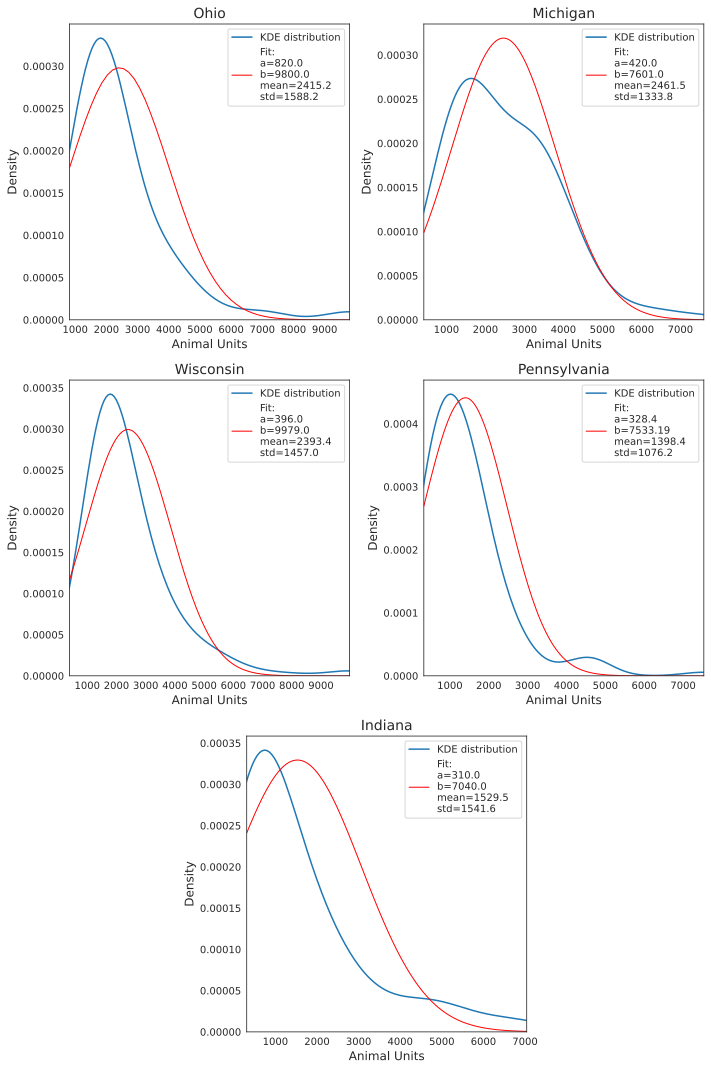
\includegraphics[width=0.81\linewidth, trim={0cm 0cm 0cm 0cm},clip]{SupMat_Figures/CAFOs_Size_Distribution} 
%	\caption{Distribution of CAFOs size in regions of the the Great Lakes area.}
%	\label{fig:CAFOsSizeDist}
%\end{figure}

\newpage
	
%\bibliographystyle{apacite}
%\bibliographystyle{ieee}
\bibliography{references}
	
\end{document}